\documentclass[10pt,a4paper]{article}
\usepackage[margin=24mm,top=21mm,bottom=22mm]{geometry}
\usepackage[T1]{fontenc}
\usepackage{lmodern,amsmath,booktabs,array,hyperref,xcolor}
\usepackage{tikz}
\usetikzlibrary{arrows.meta}
\tikzset{panel/.style={draw=link!70, rounded corners=2pt, align=center,
  fill=link!5, inner sep=4pt, font=\small, minimum height=10mm},
  arr/.style={-{Stealth[length=4pt]}, draw=link, thick}}
\newcommand{\diagramcaption}[2]{\par\smallskip{\small\textbf{Figure #1.} #2}\par}
\definecolor{link}{HTML}{245E72}
\hypersetup{colorlinks=true,urlcolor=link,linkcolor=link,pdftitle={DL Complexity: One Interface, Different Measures of Deep Learning Model Complexity}}
\setlength{\parindent}{0pt}\setlength{\parskip}{5pt}\setlength{\emergencystretch}{2em}
\newcommand{\code}[1]{\texttt{#1}}
\begin{document}
\begin{center}
{\LARGE\bfseries DL Complexity:}\par
{\Large One Interface, Different Measures of\par Deep Learning Model Complexity}\par
\medskip Alyabushev, Dementiev, Kurdyukov, Chirkov\par

\end{center}
\section*{Abstract}
Complexity measures for neural networks differ in their inputs, assumptions and scales, which makes them difficult to evaluate side by side. We present DL Complexity, a PyTorch library that evaluates a trained model through a common interface and preserves the units of each estimate. The library covers information criteria, Bayesian approximations, two-part and prequential description lengths, and compression-based risk bounds. We validate BIC against an analytical Gaussian reference and examine the effect of weight precision on a two-part code. For a fixed four-class network, six-bit quantization minimizes the combined model and label length over precisions from one to sixteen bits per index.
\section{Introduction}
Which of two trained models is more complex? Parameter count assigns a tie to every checkpoint of the same architecture. Description length offers a way to distinguish them: a compact representation saves bits on the weights, while the probabilities assigned by the decoded network determine the cost of describing the labels [1]. A compression bound asks how the size of a family of decoded classifiers limits their population risk [2].

\subsection*{Contributions}
\begin{enumerate}
\setlength{\itemsep}{1pt}\setlength{\parsep}{0pt}
\item We define a common PyTorch interface for evaluating a trained model. Each estimate carries its units, normalization and statistical assumptions, so the caller can distinguish a criterion score, a description length and a risk guarantee.
\item We separate the preparation of evidence from its evaluation. Classical criteria can reuse one likelihood pass. For lossy compression, the model codec supplies the bytes to be counted and the decoded predictor used to score the labels.
\item We provide two reproducible checks of the interface: recovery of the closed-form Gaussian BIC through two input routes, and a fixed-network precision sweep that separates storage savings from the predictive cost of quantization.
\end{enumerate}
\section{Methods}
\textbf{Library design.} A \code{ModelContext} pairs a model with its likelihood, and a \code{DataSource} supplies the observations. Each estimator checks its input requirements and returns a structured \code{ComplexityResult}. A \code{ComplexitySuite} evaluates several estimators together (Figure~1). Fitting and posterior sampling are explicit.
\begin{center}
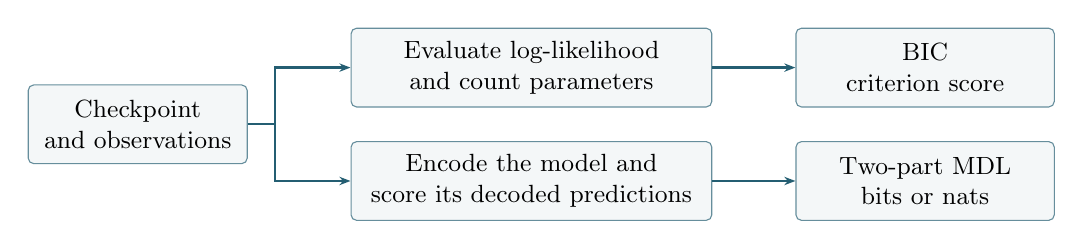
\begin{tikzpicture}
\node[panel,text width=25mm] (a) at (0,0) {Checkpoint\\and observations};
\node[panel,text width=43mm] (b) at (5,0.72) {Evaluate log-likelihood\\and count parameters};
\node[panel,text width=43mm] (c) at (5,-0.72) {Encode the model and\\score its decoded predictions};
\node[panel,text width=30mm] (d) at (10,0.72) {BIC\\criterion score};
\node[panel,text width=30mm] (e) at (10,-0.72) {Two-part MDL\\bits or nats};
\draw[arr] (a.east) -- ++(.35,0) |- (b.west);
\draw[arr] (a.east) -- ++(.35,0) |- (c.west);
\draw[arr] (b) -- (d); \draw[arr] (c) -- (e);
\end{tikzpicture}
\diagramcaption{1}{Two estimators applied to the same checkpoint. Their inputs and output scales follow from the statistical question.}
\end{center}
\newpage
For illustration, consider a linear classifier with four zero-valued parameters and four binary labels. It assigns equal probability to both classes. We evaluate BIC and request the two-part code in bits.
{\small
\begin{verbatim}
stats = prepare_fit_statistics(context, data=data)
coded = prepare_two_part(context, data=data, codec=BinaryModelCodec())
suite = ComplexitySuite({"bic": BIC(), "two_part": TwoPartMDL(unit="bits")})
report = suite.estimate(context=context, data=data,
                        inputs={"bic": stats, "two_part": coded})
for name, outcome in report.items():
    q = outcome.result.primary
    print(name, f"{q.value.item():.2f}", q.unit)
\end{verbatim}
\textit{Output}
\begin{verbatim}
bic 11.09 native_ic
two_part 3140.00 bits
\end{verbatim}
}
BIC reports a score on its native criterion scale. The two-part code uses 3,136 bits for the serialized model and one bit for each of the four labels.
\subsection*{Measures and their scales}
\textbf{Information criteria.} For total fitted log-likelihood $\ell$, parameter dimension $k$ and $n$ observations, AIC, BIC and HQIC add $2k$, $k\ln n$ and $2k\ln\ln n$, respectively, to $-2\ell$. Their outputs retain the native criterion scale. The textbook interpretation of BIC assumes regular maximum-likelihood asymptotics [3]. At arbitrary neural-network weights the formula remains computable, while the interpretation needs a separate justification.

For WAIC2, let $\ell_{si}$ be the log-likelihood of observation $i$ under posterior draw $s$. The implementation computes
\[
 -2\left[\sum_i \log\!\left(\tfrac1S\sum_s e^{\ell_{si}}\right)
       - \sum_i {\rm Var}_{s}(\ell_{si})\right],
\]
with sample variance over draws. WBIC estimates expected total negative log-likelihood (NLL) under a posterior with inverse temperature $1/\ln n$ [4]. Posterior draws can be obtained by unadjusted Langevin sampling (ULA), its Metropolis-adjusted variant (MALA) or stochastic-gradient Langevin dynamics (SGLD). Both estimates depend on how well the sampled chains represent their target distributions.

\textbf{Bayesian approximations.} The variational objective adds expected NLL under a supplied weight distribution to its KL divergence from the prior [5]. The Laplace calculation uses a local Gaussian approximation around a supplied mode and accepts Kronecker-factored curvature [6]. Exact factor preparation is available for a single Gaussian linear layer. For more general models, the user supplies the factors. Both calculations report their terms in nats.

\textbf{Prequential coding.} A prequential code charges an initial label block and then the log loss on successive blocks under predictions made before their labels are used for fitting [7] (Figure 2). Blockwise, online and uniform-prefix replay variants are implemented, with optional temperature calibration. The ledger records which prefix was available at each prediction. Training on successive prefixes can dominate the computational cost of a prequential estimate.

\begin{center}
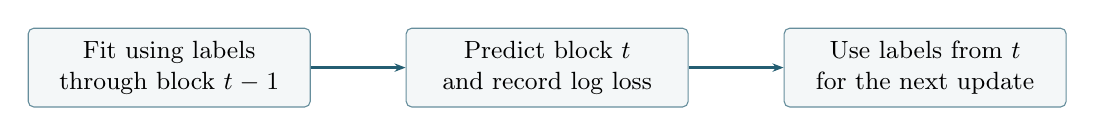
\begin{tikzpicture}
\node[panel,text width=33mm] (a) at (0,0) {Fit using labels\\through block $t-1$};
\node[panel,text width=33mm] (b) at (4.8,0) {Predict block $t$\\and record log loss};
\node[panel,text width=33mm] (c) at (9.6,0) {Use labels from $t$\\for the next update};
\draw[arr] (a) -- (b); \draw[arr] (b) -- (c);
\end{tikzpicture}
\diagramcaption{2}{One prequential step after the initial block. Each label is scored under a prediction made before that label is available for fitting.}
\end{center}
\newpage
\textbf{Model and label codes.} For a binary model message $m$ and its decoded predictor $g_m$, the discrete two-part code in bits is
\[
 L_{2\mathrm{P}}=8\,|m|_{\rm bytes}-\sum_{i=1}^{n}\log_2 p_{g_m}(y_i\mid x_i).
\]
As shown in Figure 3, the first term is measured on serialized bytes, including architecture metadata, masks, factors, quantization scales and padding as appropriate. The second is the ideal conditional label length. The codec supports dense storage, magnitude pruning with sparse storage, low-rank factors for weight matrices, and uniform quantization. Scoring the decoded model charges the predictive cost of a lossy representation.

\begin{center}
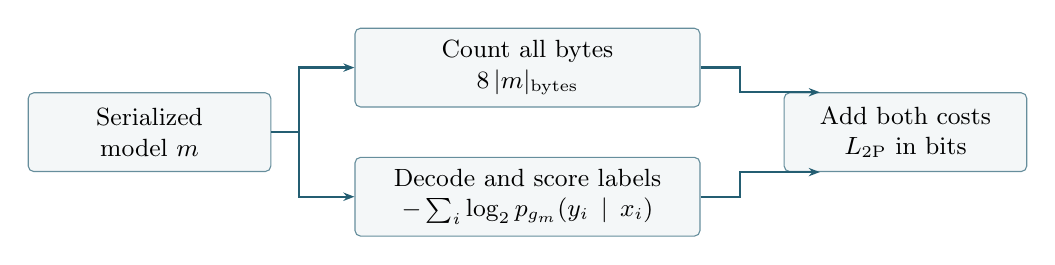
\begin{tikzpicture}
\node[panel,text width=28mm] (a) at (0,0) {Serialized\\model $m$};
\node[panel,text width=41mm] (b) at (4.8,.82) {Count all bytes\\$8\,|m|_{\rm bytes}$};
\node[panel,text width=41mm] (c) at (4.8,-.82) {Decode and score labels\\$-\sum_i \log_2 p_{g_m}(y_i\mid x_i)$};
\node[panel,text width=28mm] (d) at (9.6,0) {Add both costs\\$L_{2\mathrm{P}}$ in bits};
\draw[arr] (a.east) -- ++(.35,0) |- (b.west);
\draw[arr] (a.east) -- ++(.35,0) |- (c.west);
\draw[arr] (b.east) -- ++(.5,0) |- (d.155);
\draw[arr] (c.east) -- ++(.5,0) |- (d.205);
\end{tikzpicture}
\diagramcaption{3}{Accounting for lossy compression. Changing the precision changes the stored bytes and can also change the probabilities assigned to the observed labels.}
\end{center}
\textbf{Compression and population risk.} For independent, identically distributed observations, suppose the decoder and its family of at most $r^q$ classifiers are fixed independently of the sample. If the largest coordinatewise logit error between $f$ and $g$ on the full training sample is at most $\gamma/2$, the implemented form of Theorem 2.1 of [2] gives, with confidence $1-\delta$,
\[
 R(g)\leq \widehat L_\gamma(f)+\sqrt{(q\ln r+\ln(1/\delta))/(2n)}.
\]
Here $\widehat L_\gamma$ is the fraction of training examples whose multiclass margin is at most $\gamma$. The Matrix-Project construction encodes the weights of supported bias-free ReLU networks using indices from a finite alphabet. The result concerns the decoded predictor; a value above one is vacuous. The cardinality argument requires an explicit finite family and a pointwise evaluation rule.
\section{Experimental setup}
We consider two settings. The first has an exact solution: four observations $y=(1,2,4,5)$ from a Gaussian model with unknown mean and known unit variance. We evaluate BIC from the model and observations and independently from the sufficient statistics.

The second holds a network and its data fixed while varying only the precision of its weights. An $8$--$32$--$32$--$4$ ReLU network defines class probabilities on 20,000 independent standard Gaussian input vectors. For each input we draw one of the four labels from the network's softmax distribution. The generator for parameters, inputs and labels uses seed zero. We encode the same network at each integer precision from one to sixteen bits per index. We measure the serialized model size and evaluate the conditional label length after decoding.
\newpage
\section{Results}
\textbf{BIC against an analytical reference.} The maximum-likelihood estimate is $\hat\mu=3$, giving a residual sum of squares of 10. With $n=4$ and $k=1$, BIC is $4\ln(2\pi)+10+\ln 4\simeq18.7378$. Both evaluation routes recover this value.

\textbf{Effect of quantization.} The shortest total description occurs at six bits per index (Table~1). Going from four to six bits reduces the cost of the labels by 8,773 bits at a cost of 2,992 extra model bits. Increasing precision to eight bits saves only another 470 label bits while adding 3,008 model bits.
\begin{center}
\small\begin{tabular}{rrrr}
\toprule Bits per index & Model bits & Label bits & Total bits\\\midrule
4 & 18,800 & 14,290 & 33,090\\
6 & 21,792 & 5,517 & 27,309\\
8 & 24,800 & 5,047 & 29,847\\\bottomrule
\end{tabular}\\[3pt]
Table 1. Measured model cost and ideal label cost, rounded to whole bits.
\end{center}
\section{Discussion and limitations}
The precision sweep distinguishes representations of a single architecture that parameter count treats identically. The optimum depends on the number of observations: the model is sent once, whereas each further label adds to the conditional code length. The example measures this trade-off on a sample drawn from one teacher. Establishing whether a measure tracks generalization across architectures requires independent test data.

The resulting study can compare the Spearman rank correlation of each measure with held-out negative log-likelihood or with the gap between mean test and training negative log-likelihood. Common data splits and training budgets allow parameter count to serve as a baseline. For a compression bound, interpretation also requires a valid certificate for each decoded classifier.
\section{Conclusion}
DL Complexity makes it possible to evaluate a checkpoint as a fitted statistical model, a message to be decoded, or a classifier subject to a risk bound. Returning the units and assumptions with each result preserves these distinctions when the same model and data are used throughout. The library is available under the MIT license at the \href{https://github.com/intsystems/dl-complexity}{DL Complexity repository}.
\small
\section*{References}
\vspace{-1mm}\setlength{\parskip}{2pt}
[1] P. Gr\"unwald. \href{https://arxiv.org/abs/math/0406077}{A tutorial introduction to the minimum description length principle}. 2004.\par
[2] S. Arora et al. \href{https://proceedings.mlr.press/v80/arora18b.html}{Stronger generalization bounds for deep nets via a compression approach}. ICML, 2018.\par
[3] G. Schwarz. \href{https://doi.org/10.1214/aos/1176344136}{Estimating the dimension of a model}. Annals of Statistics, 1978.\par
[4] S. Watanabe. \href{https://jmlr.org/papers/v14/watanabe13a.html}{A widely applicable Bayesian information criterion}. JMLR, 2013.\par
[5] A. Graves. \href{https://papers.nips.cc/paper/4329-practical-variational-inference-for-neural-networks}{Practical variational inference for neural networks}. NeurIPS, 2011.\par
[6] H. Ritter, A. Botev and D. Barber. \href{https://openreview.net/forum?id=Skdvd2xAZ}{A scalable Laplace approximation for neural networks}. ICLR, 2018.\par
[7] J. Bornschein, Y. Li and M. Hutter. \href{https://arxiv.org/abs/2210.07931}{Sequential learning of neural networks for prequential MDL}. 2022.
\end{document}
